\chapter{Implementation}\label{ch:implementation}
% Prototype level
% geen documentatie manual, maar keuzes en uitdagingen

In Chapter \ref{ch:design} we proposed a generic design to enable Tribler on mobile devices.
Many types of connectible mobile devices exist.
In the context of the problem description from Chapter \ref{ch:problem_desc}, devices used for human communication, such as smart-phones, will be our prime focus.
% Why no iOS?
The largest potential user base in the smart-phone market can be reached by targeting Android OS \cite{smartphone-os}.
%Android supports multiple hardware platforms, such as ARM, x86, and x86-64.
%Most smart-phones running Android are compatible with the ARMv7 embedded application binary interface (EABI) \cite{}.
%Therefore, to reach the largest potential user base, our implementation will target Android OS on ARMv7 compatible platforms.
Therefore, our implementation will target Android OS.

Following the choice for Android, the generic design in Figure \ref{fig:system_architecture_design} can be further specified as presented in Figure \ref{fig:system_architecture_implementation}.
Two main additions are a separate video player and a Java native interface (JNI) component.
In the following sections, each component from Figure \ref{fig:system_architecture_implementation} will be described in more detail.
The complete build tool-chain is presented in Section \ref{sec:build_toolchain}, which combines everything to build the final Android application package (APK).
Finally, the statistics of the implementation are presented in Section \ref{sec:impl_stats}.

\begin{figure}[H]
	\centering
	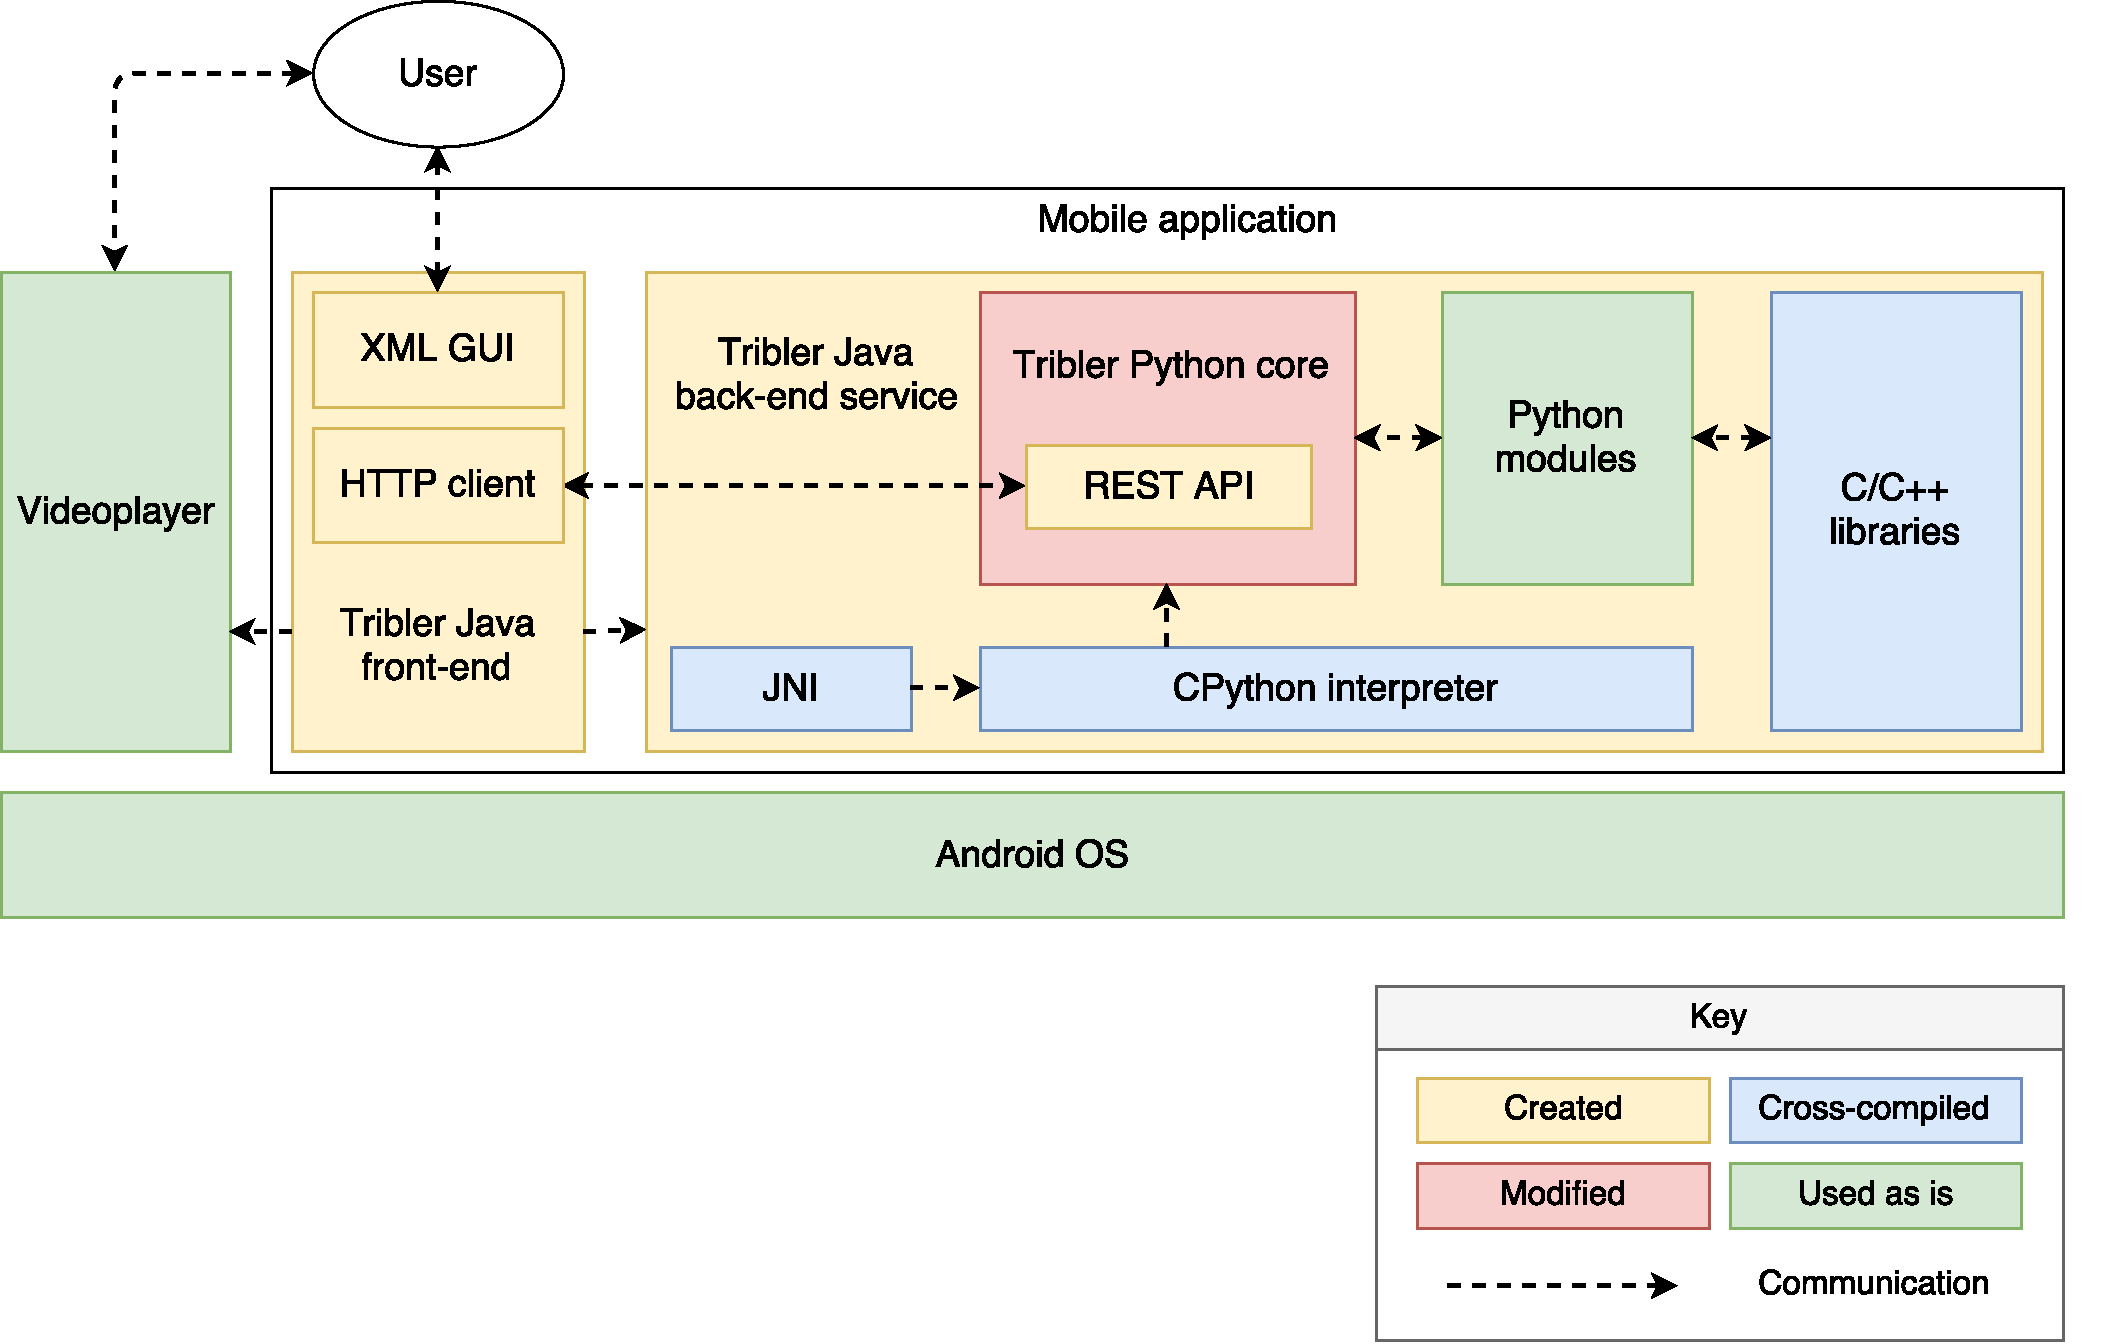
\includegraphics[width=\textwidth]{system_architecture_implementation}
	\caption{Implemented system architecture}
	\label{fig:system_architecture_implementation}
\end{figure}


\section{Android OS}
Android is an operating system, based on the Linux kernel, that runs on smart-phones, tables, wearables and smart-TVs.
It provides a Java Virtual Machine (VM) and a Java application framework API.

Since API version 14, near field communication (NFC) and Wi-Fi peer-to-peer (P2P) connections between compatible devices is supported.
And since API version 16, a NFC push message can be used to start large file transfers over Bluetooth (req. \ref{rq:BeamApp}).
This can be used in the context of the problem description, for Tribler needs to be able to spread wireless from phone to phone.
Using this NFC push message functionality, the transfer of the APK file is fully automated (req. \ref{rq:P2P}).
Figure \ref{fig:beam} shows the instructions for the user of this effortless transfer: just hold the phones back to back.
Bluetooth, rather than Wi-Fi, is the technology of choice here, because the former has a standard file transfer protocol, built into Android OS, and the latter does not.
This means there are no prerequisites on the receiving device for receiving and installing Tribler from a nearby phone via NFC+Bluetooth.
If NFC is not available, all other options to transfer the APK are presented to the user to choose from instead.
If NFC is available, but not enabled on the device, the implementation will prompt the user to do so.
In that case, the other options are accessible via a button with the Bluetooth icon on the action bar.
NFC is used to enable easy sharing of channels as well, for example your own channel or your favorites.
After receiving the NFC push message, Tribler is automatically started and asks the user if the received channel must be added to their favorites.

Our implementation supports API version 18 and higher, because of reasons explained in Section \ref{sec:libc}.
85.6\% of Android devices run API version 18 or higher \cite{android-dashboard}.
Android support libraries are used to abstract from differences between API versions (req. \ref{rq:SupportLibs}).

Inter-application communication, via Android intents, must be secured (req. \ref{rq:AttackResilient}) .
An Intent is a messaging object to request an action from another app component \cite{android-intents}.
Therefore, all Android intents are explicit for internal actions and the action of all received intents is checked, especially broadcast intents \cite{intent-secure}. 
Also, only the activities and services that should be publicly accessible are exported in the application manifest.


\section{Tribler Java back-end service}
Our implementation uses Java to build upon the Android Java API.
To run an application in the background, even when the screen is turned off, it must be run as a service.
Therefore, every component, except the GUI, is part of the back-end service (req. \ref{rq:Service}).
The service is started as a separate process by the Java front-end (req. \ref{rq:Responsive}).
This way the user can be presented with the GUI, that indicates the service is loading in the background (req. \ref{rq:Gui}, \ref{rq:Progressbar}).

\subsection{Tribler Python core}
Tribler is written entirely in Python, but Android does not support this natively.
Python is an interpreted language, 
Because our design requirements (\ref{rq:Independence}, \ref{rq:PythonClibs})  we incorporate a Python interpreter into our design.
On top of that the entire core of Tribler can run, containing a REST HTTP API module also written in Python.

%Re-usability is an important design objective that can greatly improve maintainability as well.
%Therefore we aim to completely re-use the Tribler core, meaning everything but the GUI.
%We focus on implementing all the features of Tribler as described Chapter \ref{ch:tribler}.


%\subsubsection{REST API}
% async front-back means rest api
All communication with the front-end is done asynchronously via a REST API (req. \ref{rq:Async}).

Finally, the REST API communicates with an HTTP Client on the user interface side via JSON.


\subsection{JNI}
Using Java requires the use of the Java native interface (JNI) to communicate with the C/C++ components.
JNI enables functions that are written in C to be callable from Java and vice-versa.
The Python interpreter is started by the Java service using JNI, after loading the necessary C/C++ libraries.
%P4A uses the Java native interface (JNI), between Java and C/C++ code, to launch the CPython interpreter from a thin Java Android application.
%This Java application contains an Android service that wraps the original P4A CPython launcher.


\subsection{CPython interpreter}
Tribler uses C++ implementation of torrent protocol, called libtorrent.
To use this C/C++ library from within Python a certain capable interpreter is required.
P4A offers such an interpreter: CPython.


% Alternatieven QT, P4A, oudere python projecten
What alternatives are there, besides P4A, to run python code on Android?
0. QPython: scripting, cannot build regular .apk
1. QtAndroid, inmiddels alternative, niet gereed toen wij hieraan werkte (juni 2016, qt 5.7 android service)
2. PGS4A: no longer in development
3. SL4A: no longer in development
% Verdedig P4A keuze
Why is P4A chosen?
% Keuze voor P4A door eerder werk en beste match (legacy)
Because this project continued from previous work (legacy code) build on P4A.
% Crosscompilen met python bindings libraries (en dependencies)
Even though the revamp version was build from scratch, it still is the best choice because it not only provides the Python interpreter, it also is a complete tool-chain to cross-compile native libraries with bindings and build a standalone Android app installation package (.apk).

\subsection{Python modules}
Tribler is written entirely in Python, but most of its dependencies are written in C/C++.
To use these libraries on a mobile device they need to be compiled for the right embedded-application binary interface (EABI) including all nonstandard dependencies.
Figure \ref{fig:dependency_tree} shows the dependency tree.

\begin{figure}[H]
	\centering
	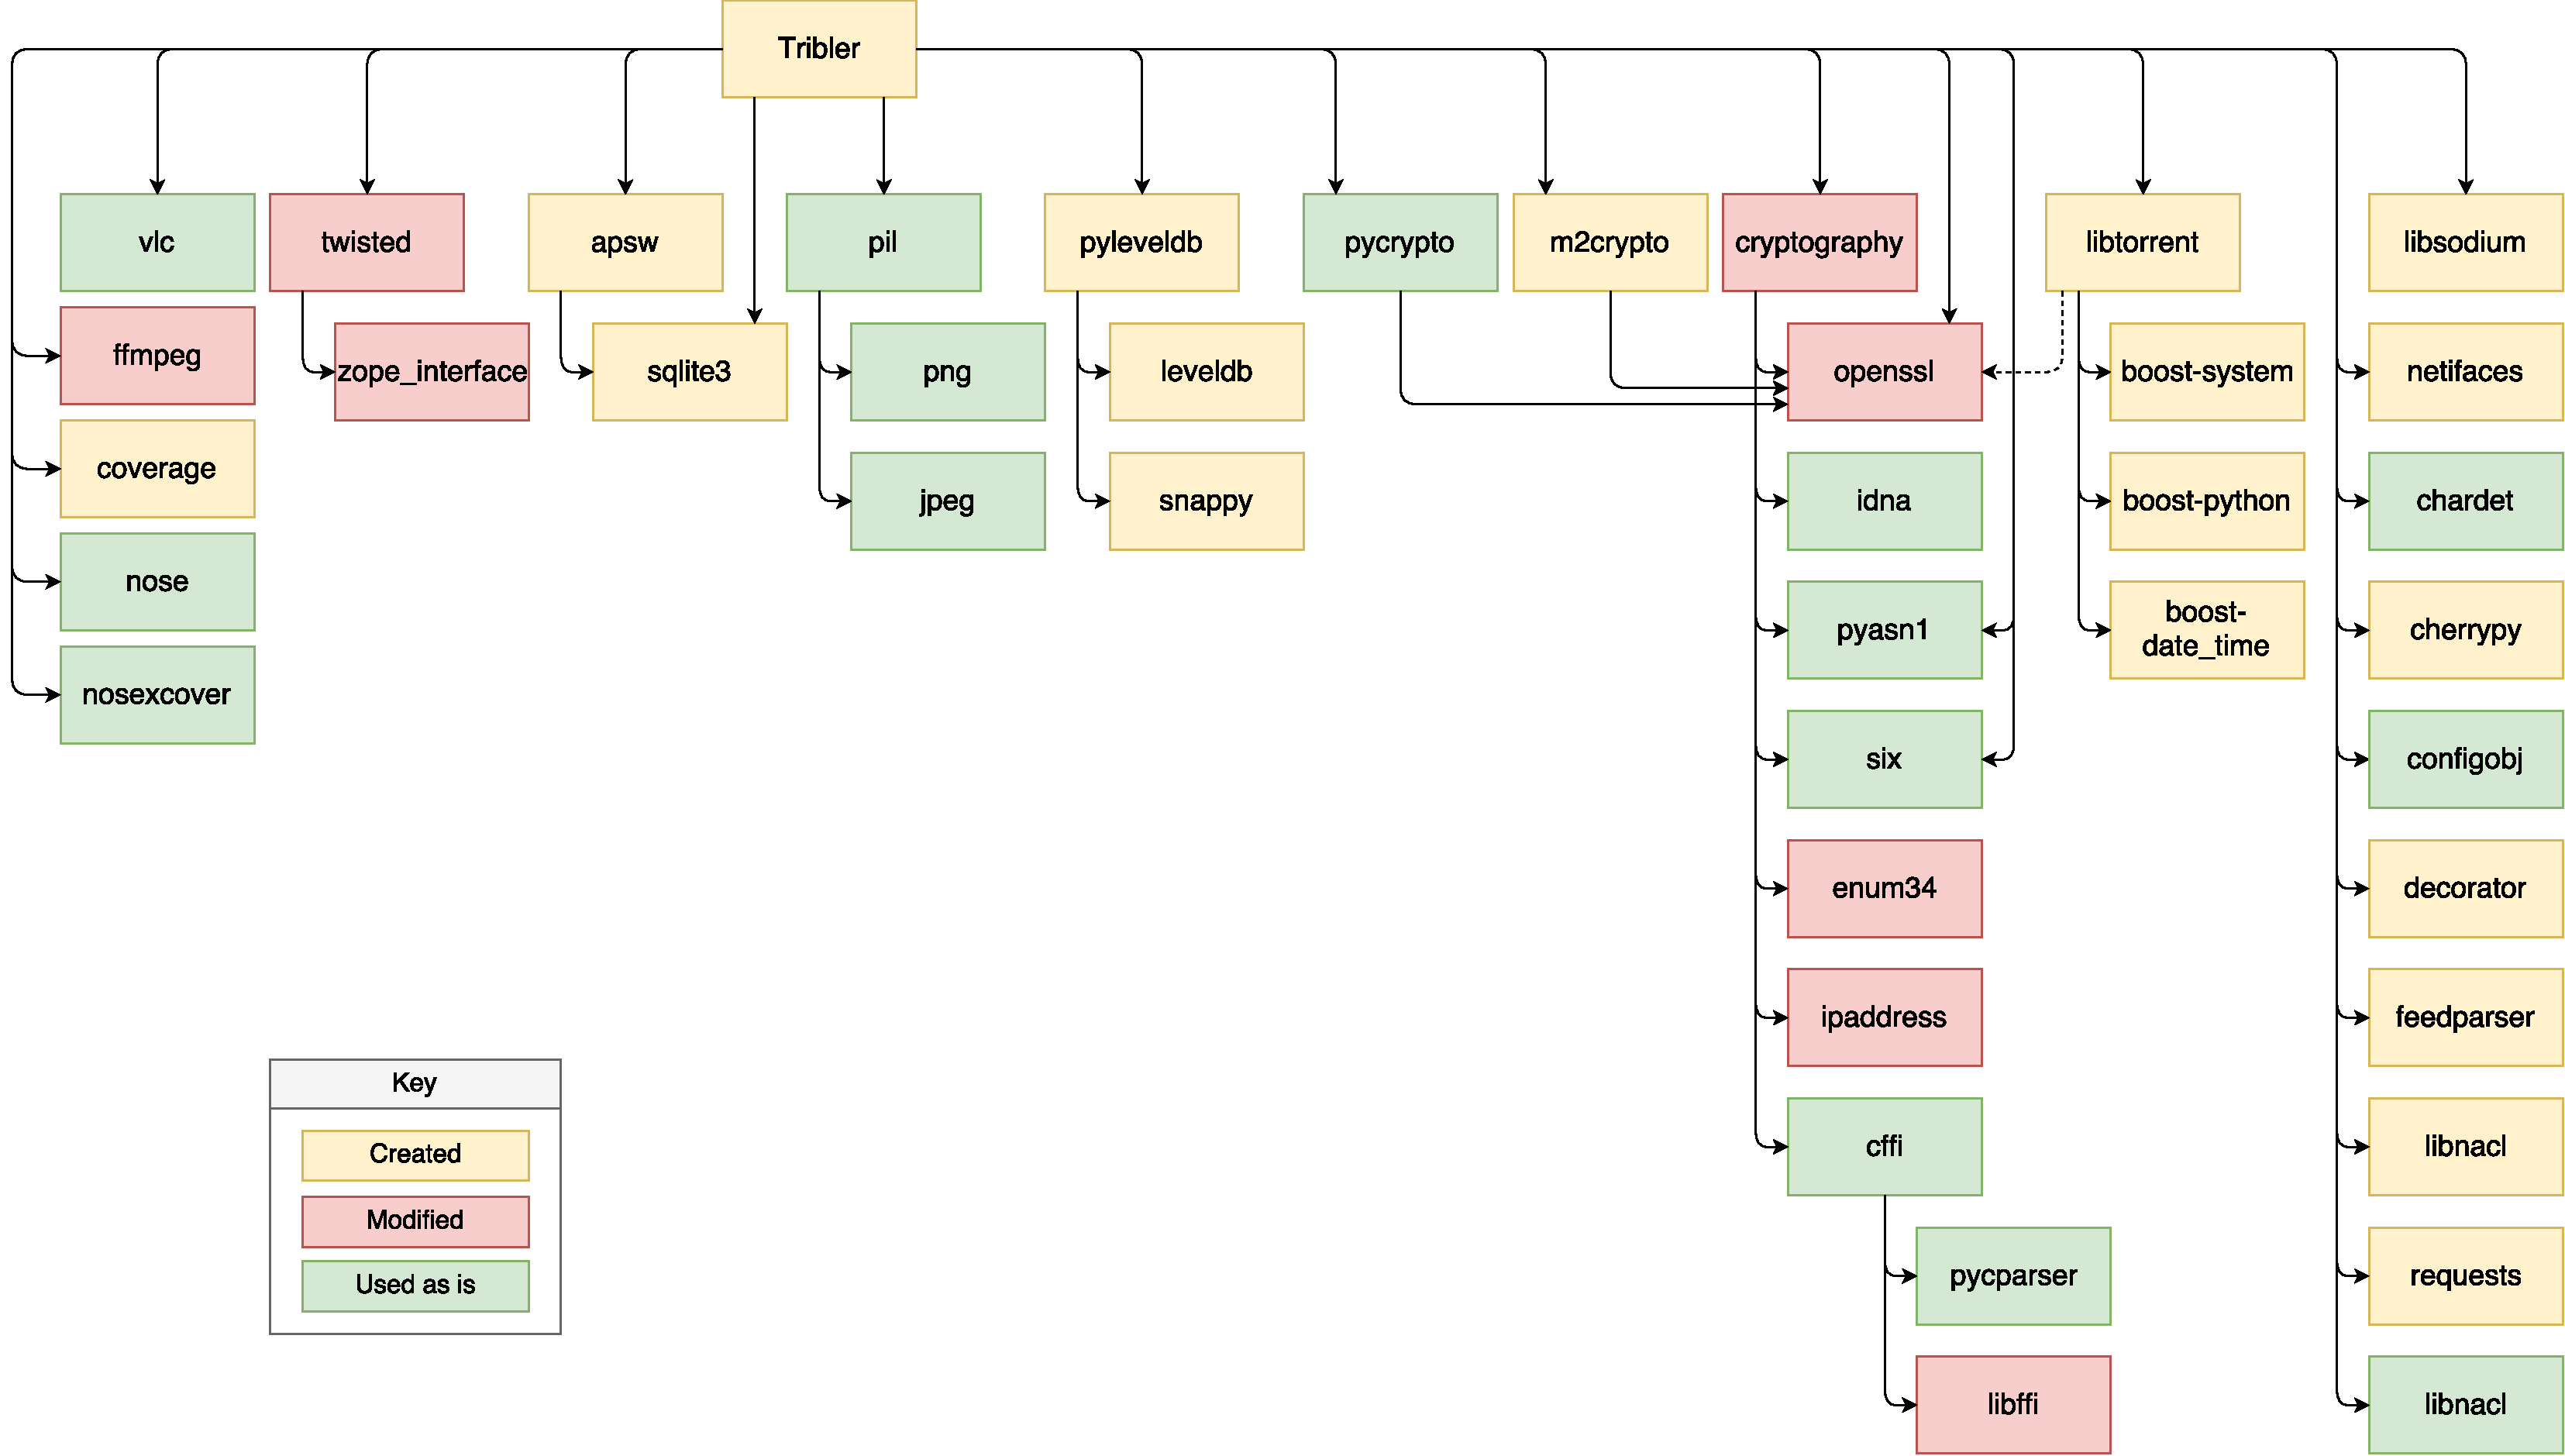
\includegraphics[width=\textwidth]{dependency_tree}
	\caption{Tribler dependencies in terms of Python-for-Android recipes}
	\label{fig:dependency_tree}
\end{figure}


\subsection{C/C++ libraries}\label{sec:libc}
The standard C library of Android differs from the GNU C Library (glibc), which makes it not trivial to port Linux libraries to Android.
All C/C++ dependencies of Tribler were therefore linked against glibc and glibc is included as a shared library (req. \ref{rq:Independence}, \ref{rq:PythonClibs}).
Static linking could result in unexpected behavior if more than one library is linked \cite{android-cpp}, and Tribler uses many, as shown in Figure \ref{fig:dependency_tree}.
Since Android 4.3 (API version 18) shared libraries do not have to be loaded in order manually anymore.
Therefore, 

The Python code loads other Python and native modules directly.

% https://kos.gd/posts/5-ways-to-use-python-with-native-code/
Calling C code directly from Python is possible by using the Python ctypes module to load a native dynamic-link library (.so files on Android) or by using the Python/C API of CPython.
This API enables a library to define functions that are written in C to be callable from Python.
These Python bindings are the glue between pure Python and pure C code.
SWIG can generate the boiler plate code for this.
Libtorrent, one of Triblers' main components, uses Boost.Python to provide a standard C++ API on top of the Python/C API.
%Kivy uses Cython, but was later dropped
% Many parts are written in C using Cython. \cite{kivy.org}
% The major alternative approach promoted by the community is best represented by Cython. Cython is a Python superset designed to be compiled down to CPython C extension modules. One of the features Cython offers (as is possible from any binary extension module) is the ability to explicitly release the GIL around a section of code. By releasing the GIL in this fashion, Cython code can fully exploit all cores on a machine for computationally intensive sections of the code, while retaining all the benefits of Python for other parts of the application. \cite{http://python-notes.curiousefficiency.org/en/latest/python3/multicore_python.html}

The Python/C API is actually so powerful it even provides access to the internals of the interpreter to mess with the global interpreter lock (GIL) which could be released during native C calls to improve the multi-threading performance of Tribler crypto.


\section{Tribler Java front-end}
The requirements on asynchronous communication (\ref{rq:Async}) and responsiveness (\ref{rq:Responsive}) require the decoupling of the GUI from the back-end.

The GUI is created by a native Android Java application, which talks to the REST API module.
The API combined with Java is better for parallelization than the coarse grained locking by the CPython interpreter.
Shared memory threading in Python code is restricted to single-thread performance because of the global interpreter lock (GIL).

Having two separate Python interpreters in distinct processes talking to each other, because that means using a very resource heavy Python GUI instead of the regular and lightweight native Android Java XML GUI.
The latter has tools available for automated UI testing.

\begin{figure}[p]
	\centering
	\begin{minipage}{.4\textwidth}
		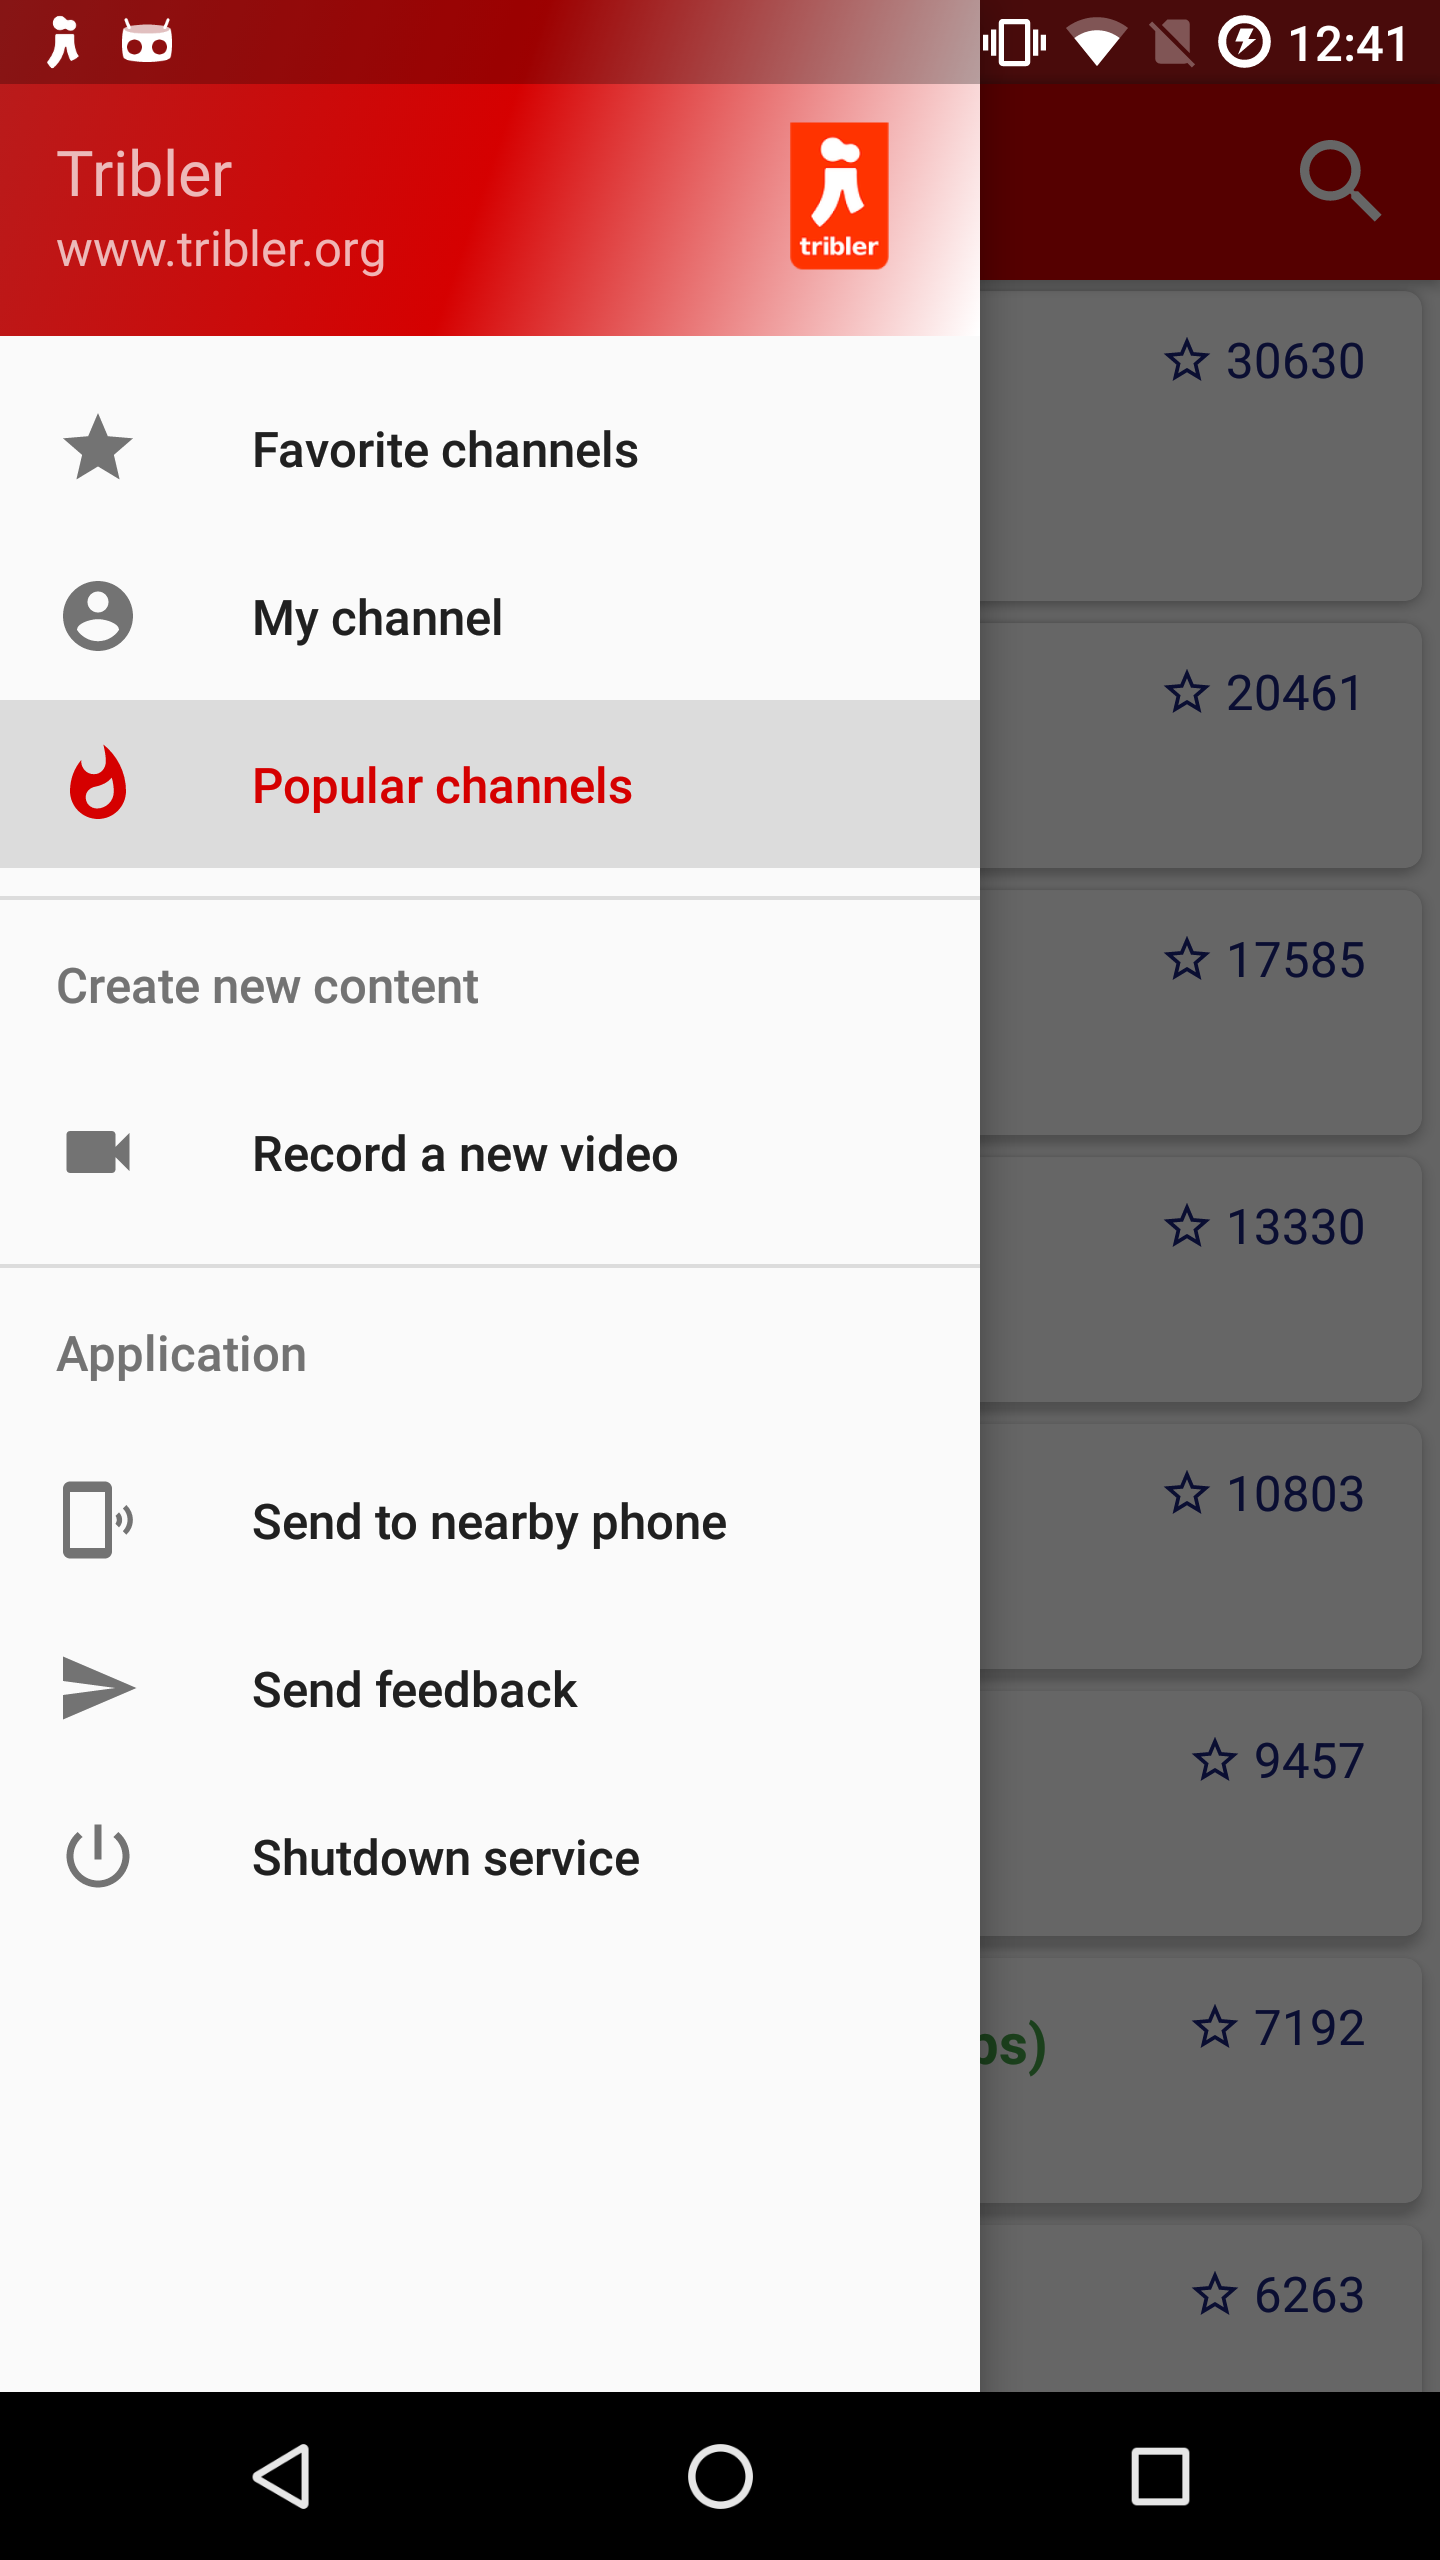
\includegraphics[width=\textwidth]{device-2016-08-28-menu-popular}
		\caption{Navigation menu of the Tribler app}
		\label{fig:menu-popular}
	\end{minipage}
	~
	\begin{minipage}{.4\textwidth}
		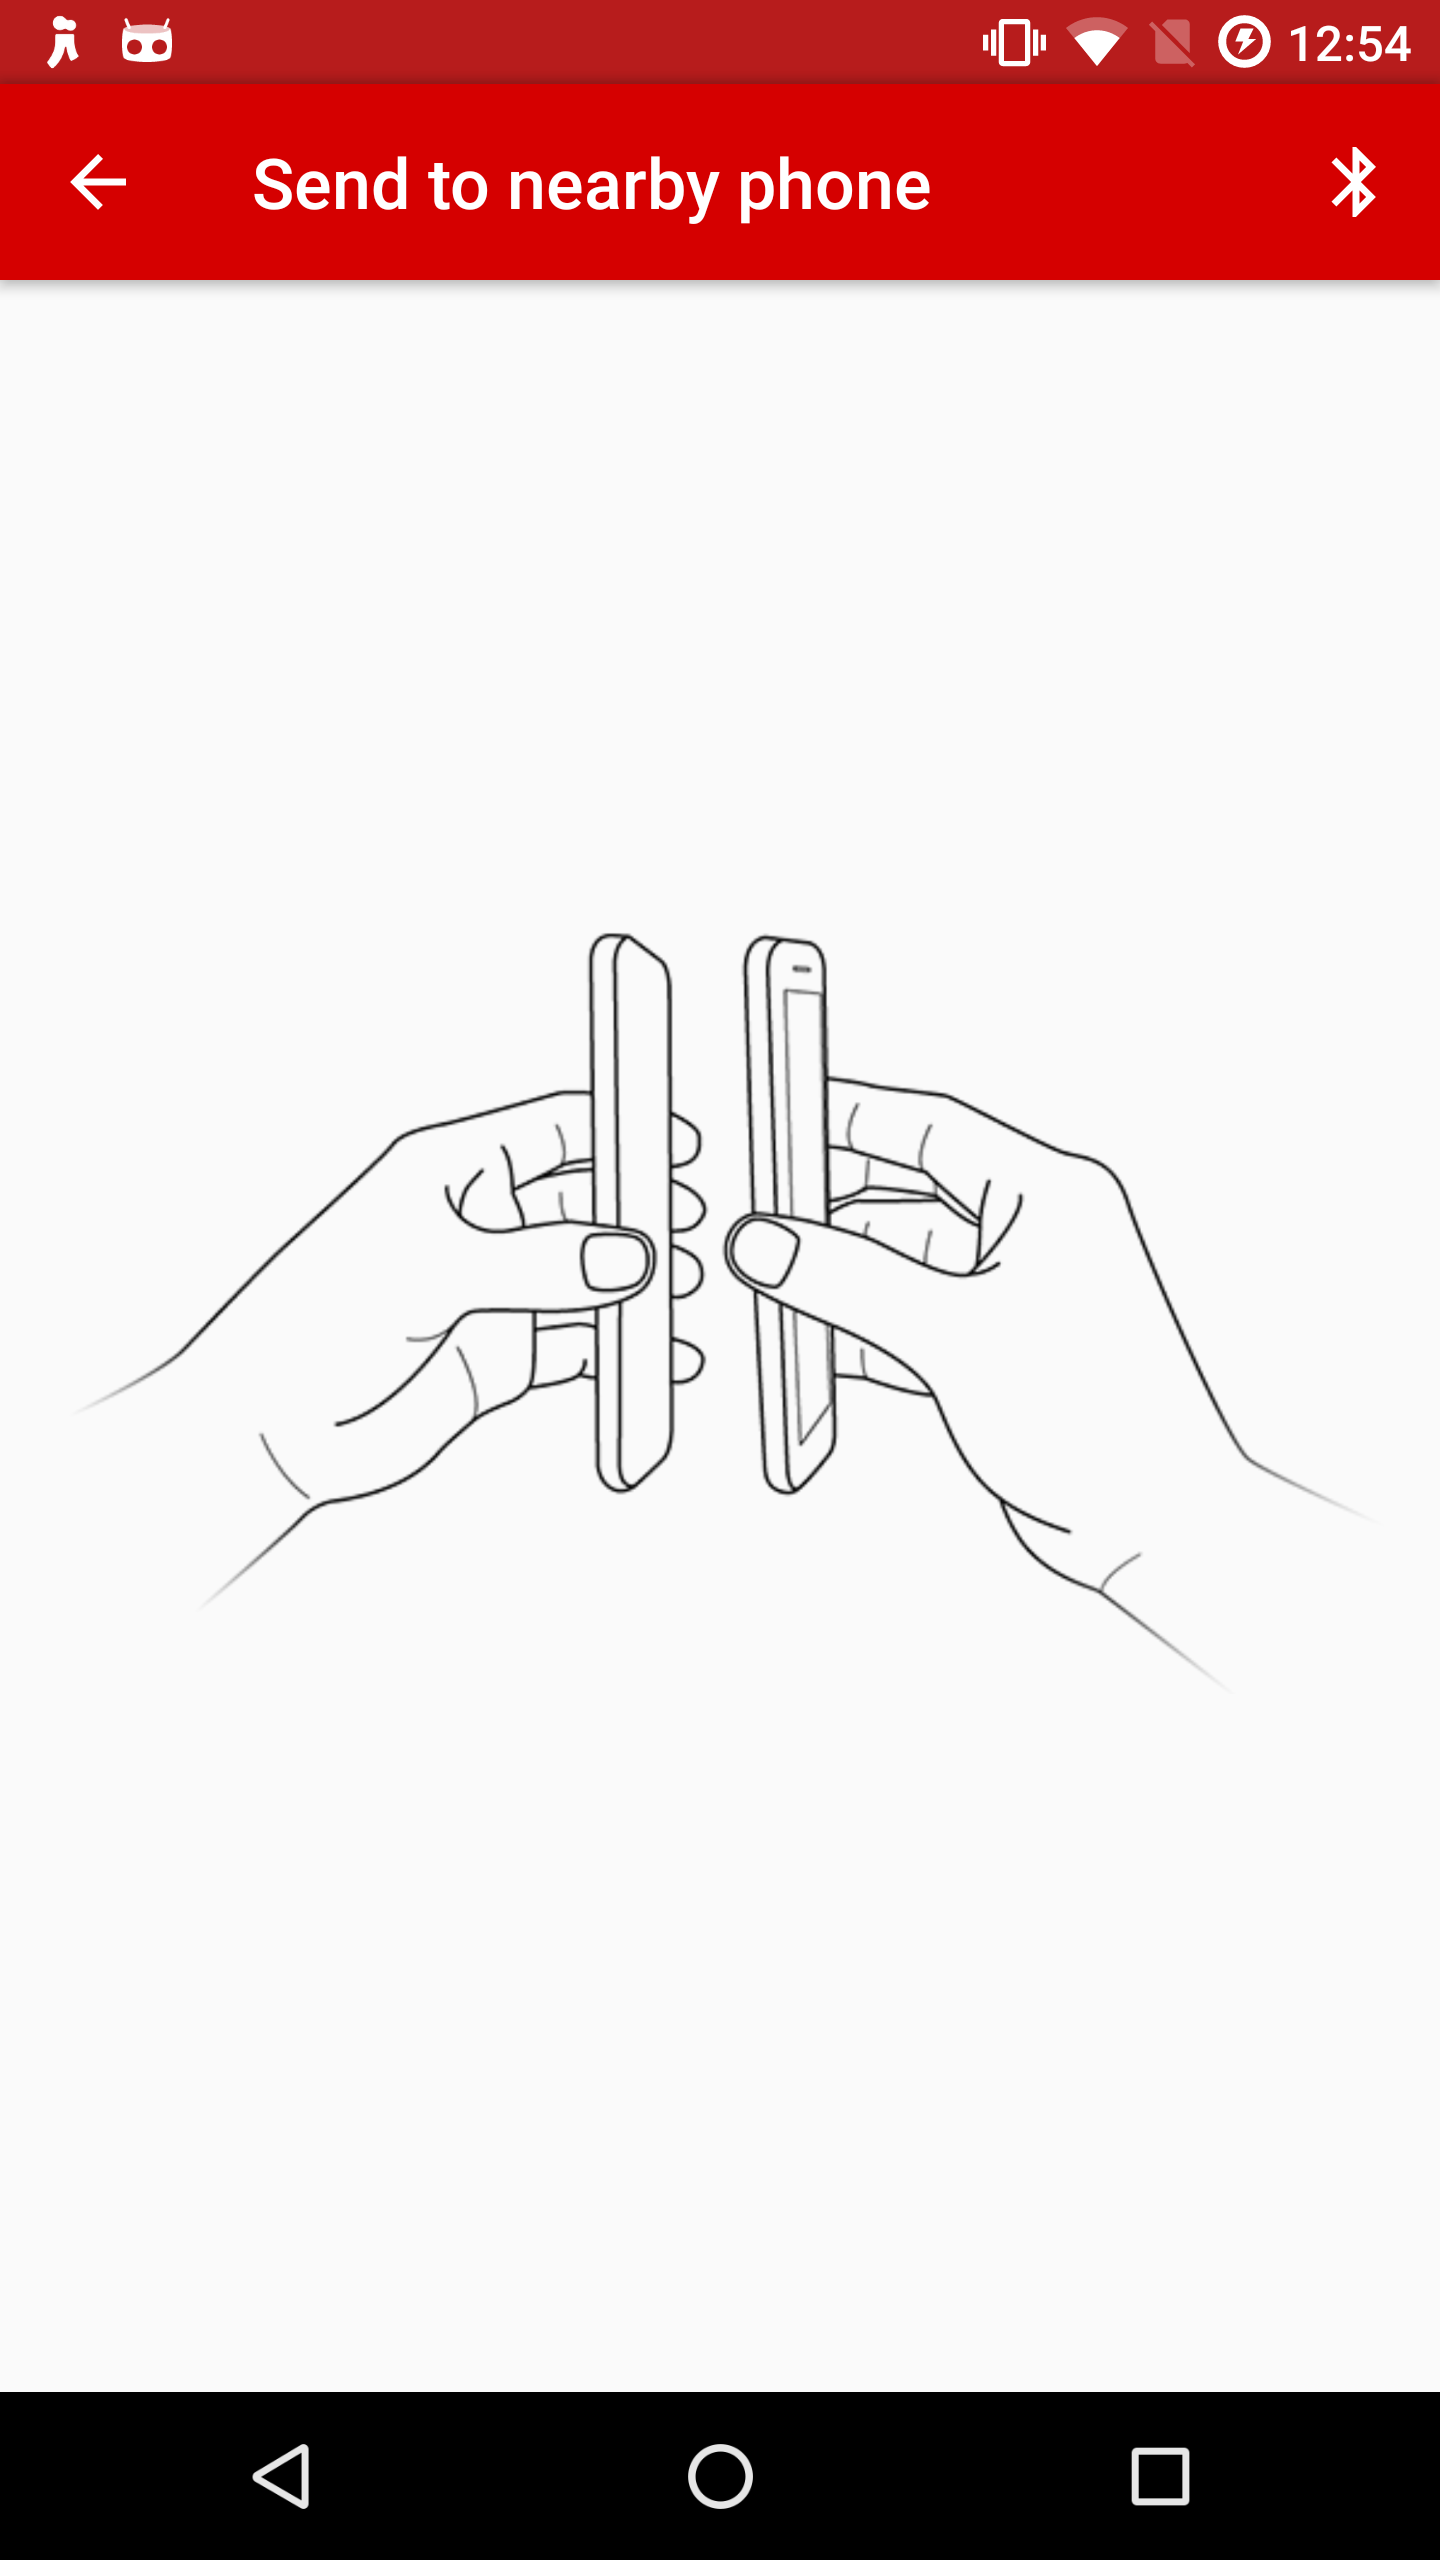
\includegraphics[width=\textwidth]{device-2016-08-28-beam}
		\caption{NFC+Bluetooth transfer of app or channel}
		\label{fig:beam}
	\end{minipage}
	
	\begin{minipage}{.4\textwidth}
		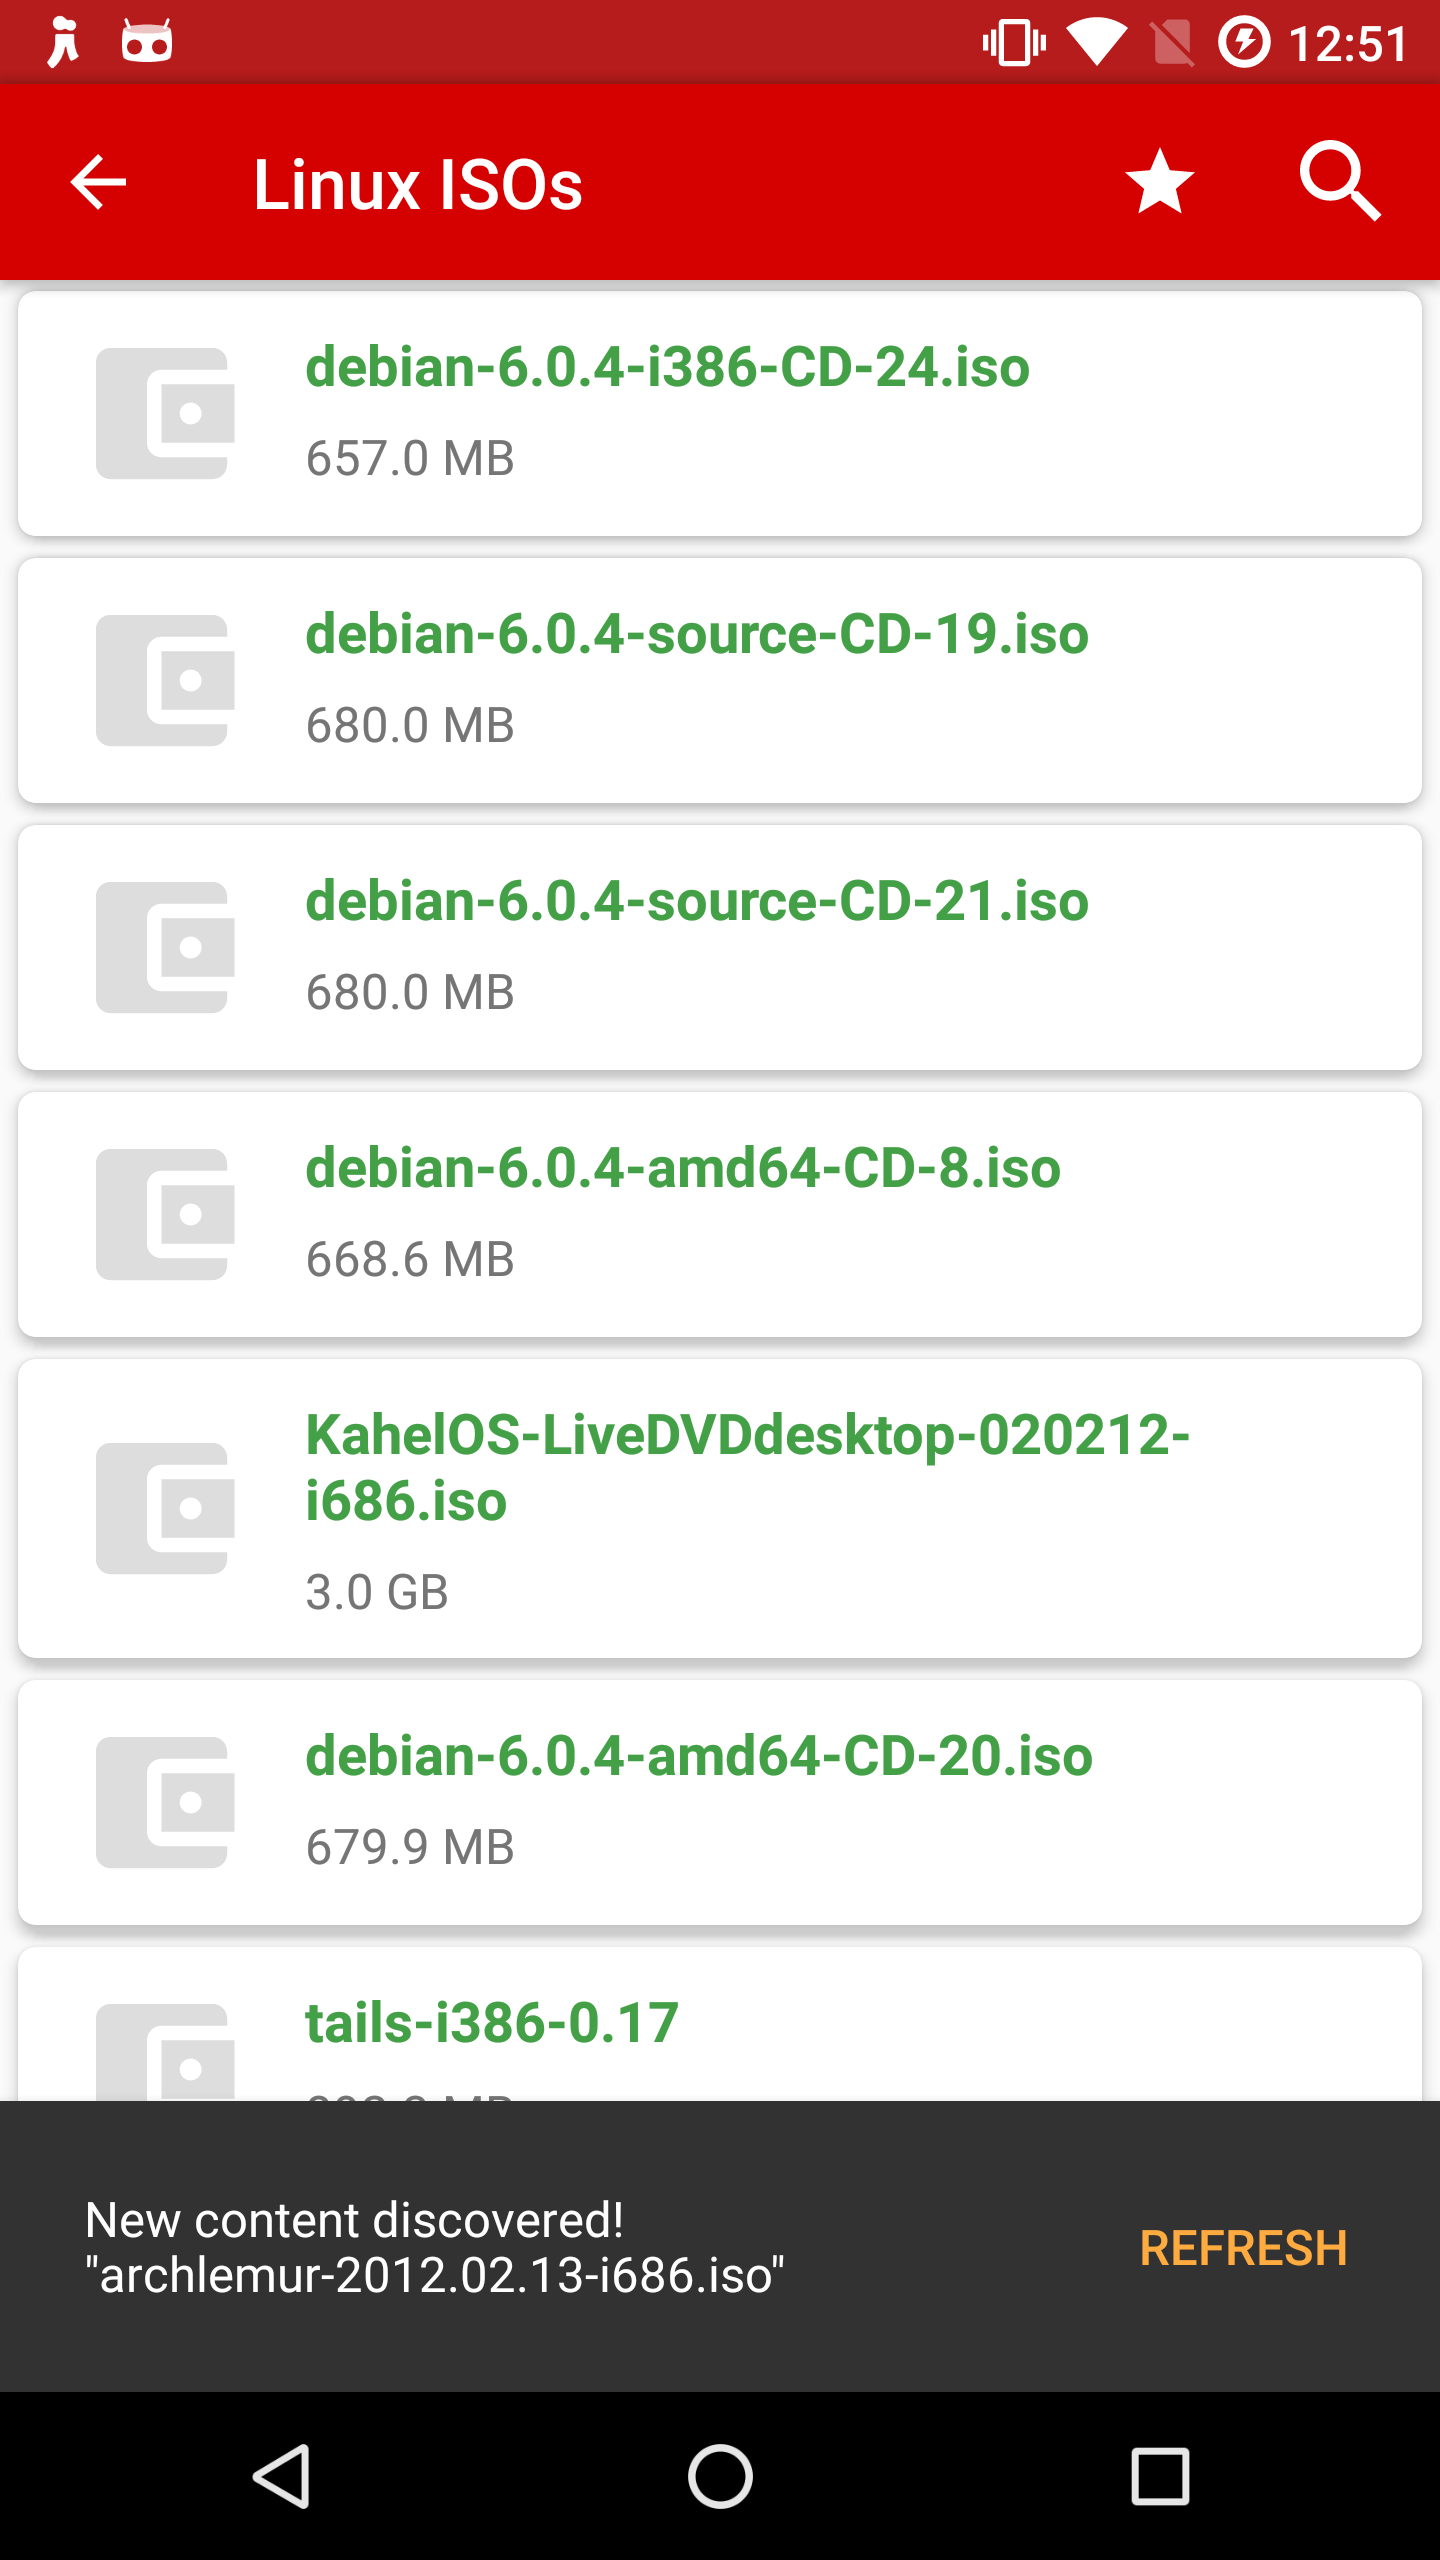
\includegraphics[width=\textwidth]{device-2016-08-28-channel-content-discovered}
		\caption{Channel with newly discovered content}
		\label{fig:channel-content-discovered}
	\end{minipage}
	~
	\begin{minipage}{.4\textwidth}
		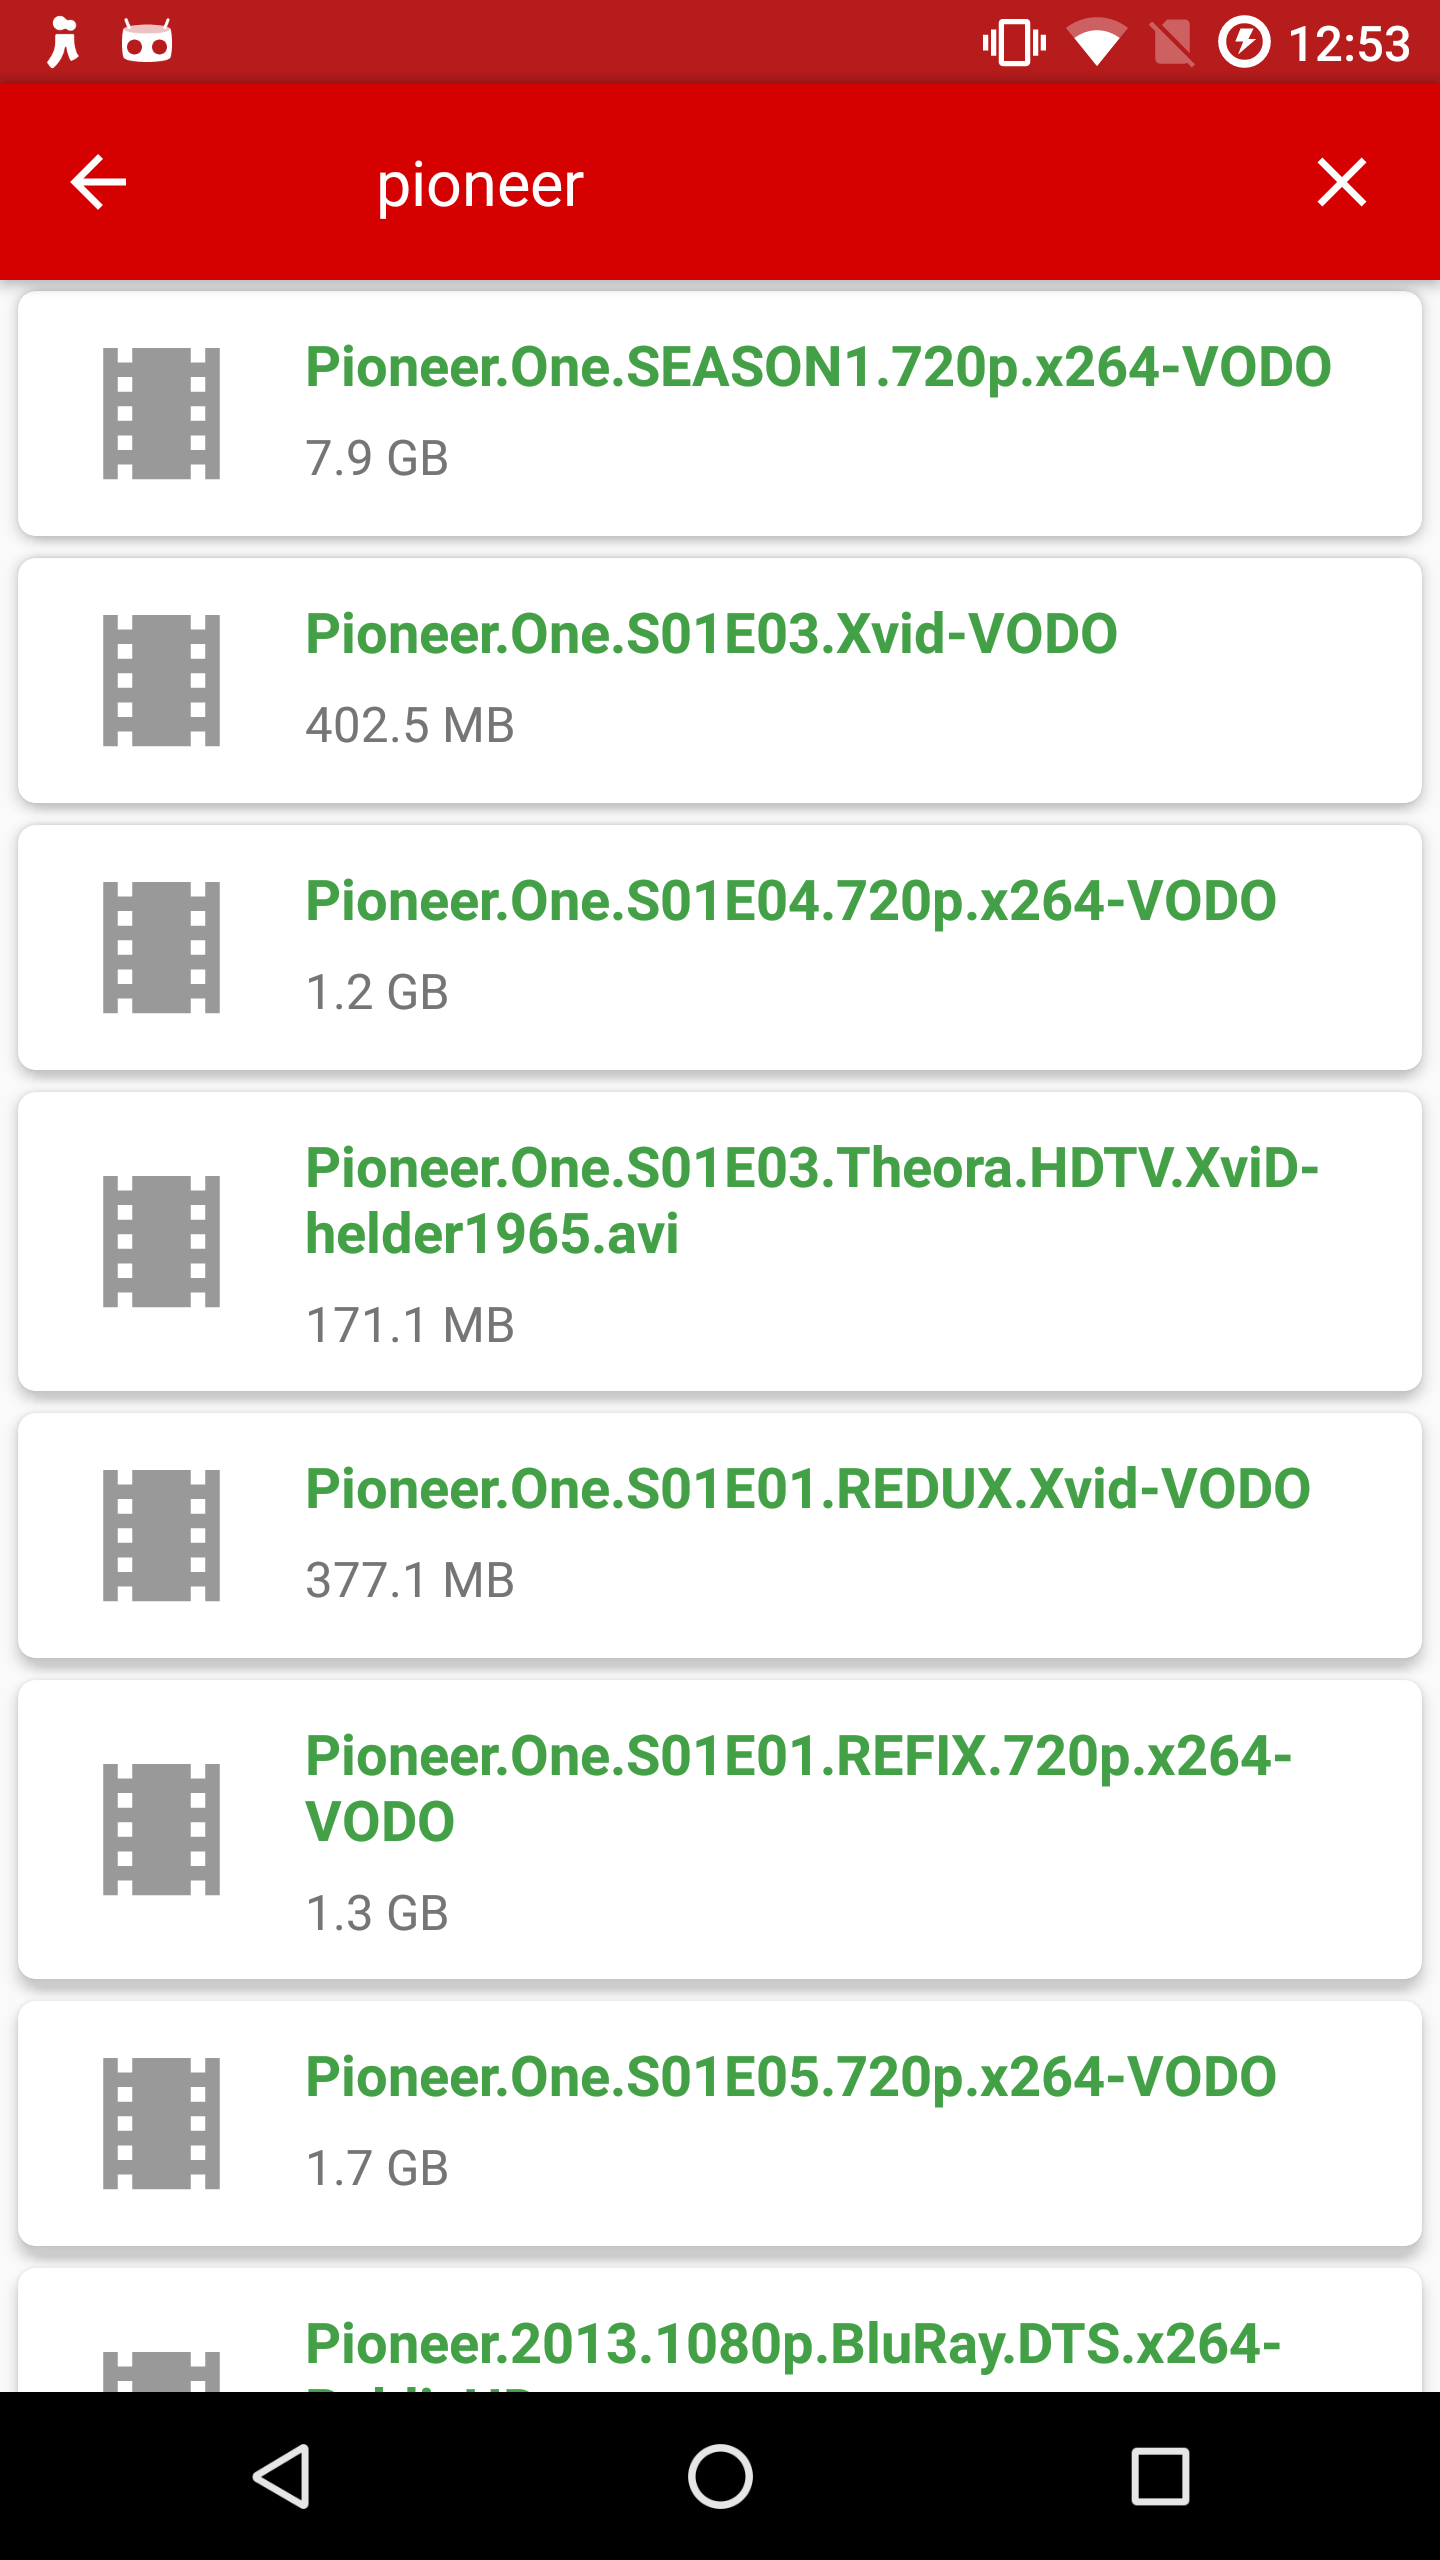
\includegraphics[width=\textwidth]{device-2016-08-28-search-pioneer}
		\caption{Search results showing video content}
		\label{fig:search-pioneer}
	\end{minipage}
\end{figure}

%The implementation of features dictated by our functional requirements in Section \ref{sec:func_req} is shown in the following screenshots.
%TODO: Figuren en REQUIREMENTS verwijzen en doorspreken

Figure \ref{fig:menu-popular} shows the main menu of the Tribler app.
The first three items presented to the user are the main views: the user's favorite channels, their own channel and discovering popular content.
The next four items are actions related to creating new content or related to the application.
It is organized this way to benefit from the simplicity of a flat menu while the actions are grouped by context with a header for clarity.

Users can browse through a list of popular channels or their own favorites.
Each channel has an indicator of the amount of users that have added that channel to their list of favorites, as can be seen behind the menu in Figure \ref{fig:menu-popular}.
Channels contain multi-media content added by their respective channel owner or everyone, depending on the security policy of that channel.
Tribler allows three settings: open, semi-open and closed.

%CHANNEL_CLOSED, CHANNEL_SEMI_OPEN, CHANNEL_OPEN, CHANNEL_MODERATOR = range(4)
%CHANNEL_ALLOWED_MESSAGES = (
%[],
%["comment", "mark_torrent"],
%["torrent", "comment", "modification", "playlist_torrent", "moderation", "mark_torrent"],
%["channel", "torrent", "playlist", "comment", "modification", "playlist_torrent", "moderation", "mark_torrent"]
%)

The favorite channels and popular channels views both show a list of channels  contain content

Search is accessible from any channel view.
Upon typing keywords into the search bar
debounce

%TODO: Describe all screenshots


\subsection{HTTP Client}
The HTTP client that talks in JSON with the REST API is build on the popular library OkHttp and fits perfectly to RxJava with a library called Retrofit.
The Retrofit library enables a very declarative API client.
%FIG code example

Because of the nature of Android to destroy interface elements if a configuration chance occurs, the asynchronous tasks running in the background must be registered and unregistered properly to avoid memory leaks.
To detect notorious memory leaks on Android we use another library made to do exactly that: LeakCanary.
Android provides a way to deal with continuity of activities with fragments that can remain in memory which were used in conjunction with composite subscriptions of RxJava.

\subsection{XML GUI} % native gui
Due to the fact that Android targets mobile devices it is very optimized for low resource usage.
Therefore memory is freed more aggressively and the application is often paused or stopped and restarted if the user switches to another app.
Running two interpreters with Python Kivy front-end and Python Tribler back-end would be doubling memory usage for the interpreter itself and require an inter-process protocol as well.
Native Java with XML front-end and Python Tribler back-end brings the user experience seamlessly in line with the native UI.

To run in the background Tribler uses an Android service and all communication is performed asynchronously.
The reactive programming paradigm is a perfect fit for asynchronous tasks.
Thanks to RxJava and RxAndroid asychronous multi-threaded coding is made very enjoyable:
%FIG code example
As shown in the code example performing IO tasks on the dedicated Android thread and making UI changes on the main thread becomes trivial.


\section{Video player}
To support streaming playback of videos (req. \ref{rq:StreamingVideo}) a capable video player is required.
The video player VLC is integrated in the desktop version of Tribler.
However, such a library, and integration of a custom GUI, is hard to maintain.
VLC is offered as a standalone Android application package (APK) from their website \cite{vlc-apk}.
Therefore, rather than implementing our own GUI, this APK is embedded as a whole inside Tribler's APK as an asset (req. \ref{rq:DistSingleApk}).
If VLC is not yet installed on the device, the user is prompted to do so and offered the version from inside Tribler.
This allows the user to install VLC without further requirements.
%The video player VLC can be integrated as hard to maintain library and a custom GUI.
%This was done first, but afterwards we decided to improve maintainability by packaging the entire Android app installation package (.apk).
%Which was also much easier to accomplish in hindsight.


\section{Build tool-chain}\label{sec:build_toolchain}
%TODO: Build toolchain beter inleiden

The Python-for-Android tool-chain uses recipes to cross compile the C/C++ libraries with Python bindings with the necessary build tools.
These recipes are like a high level make file.

\begin{figure}[H]
	\centering
	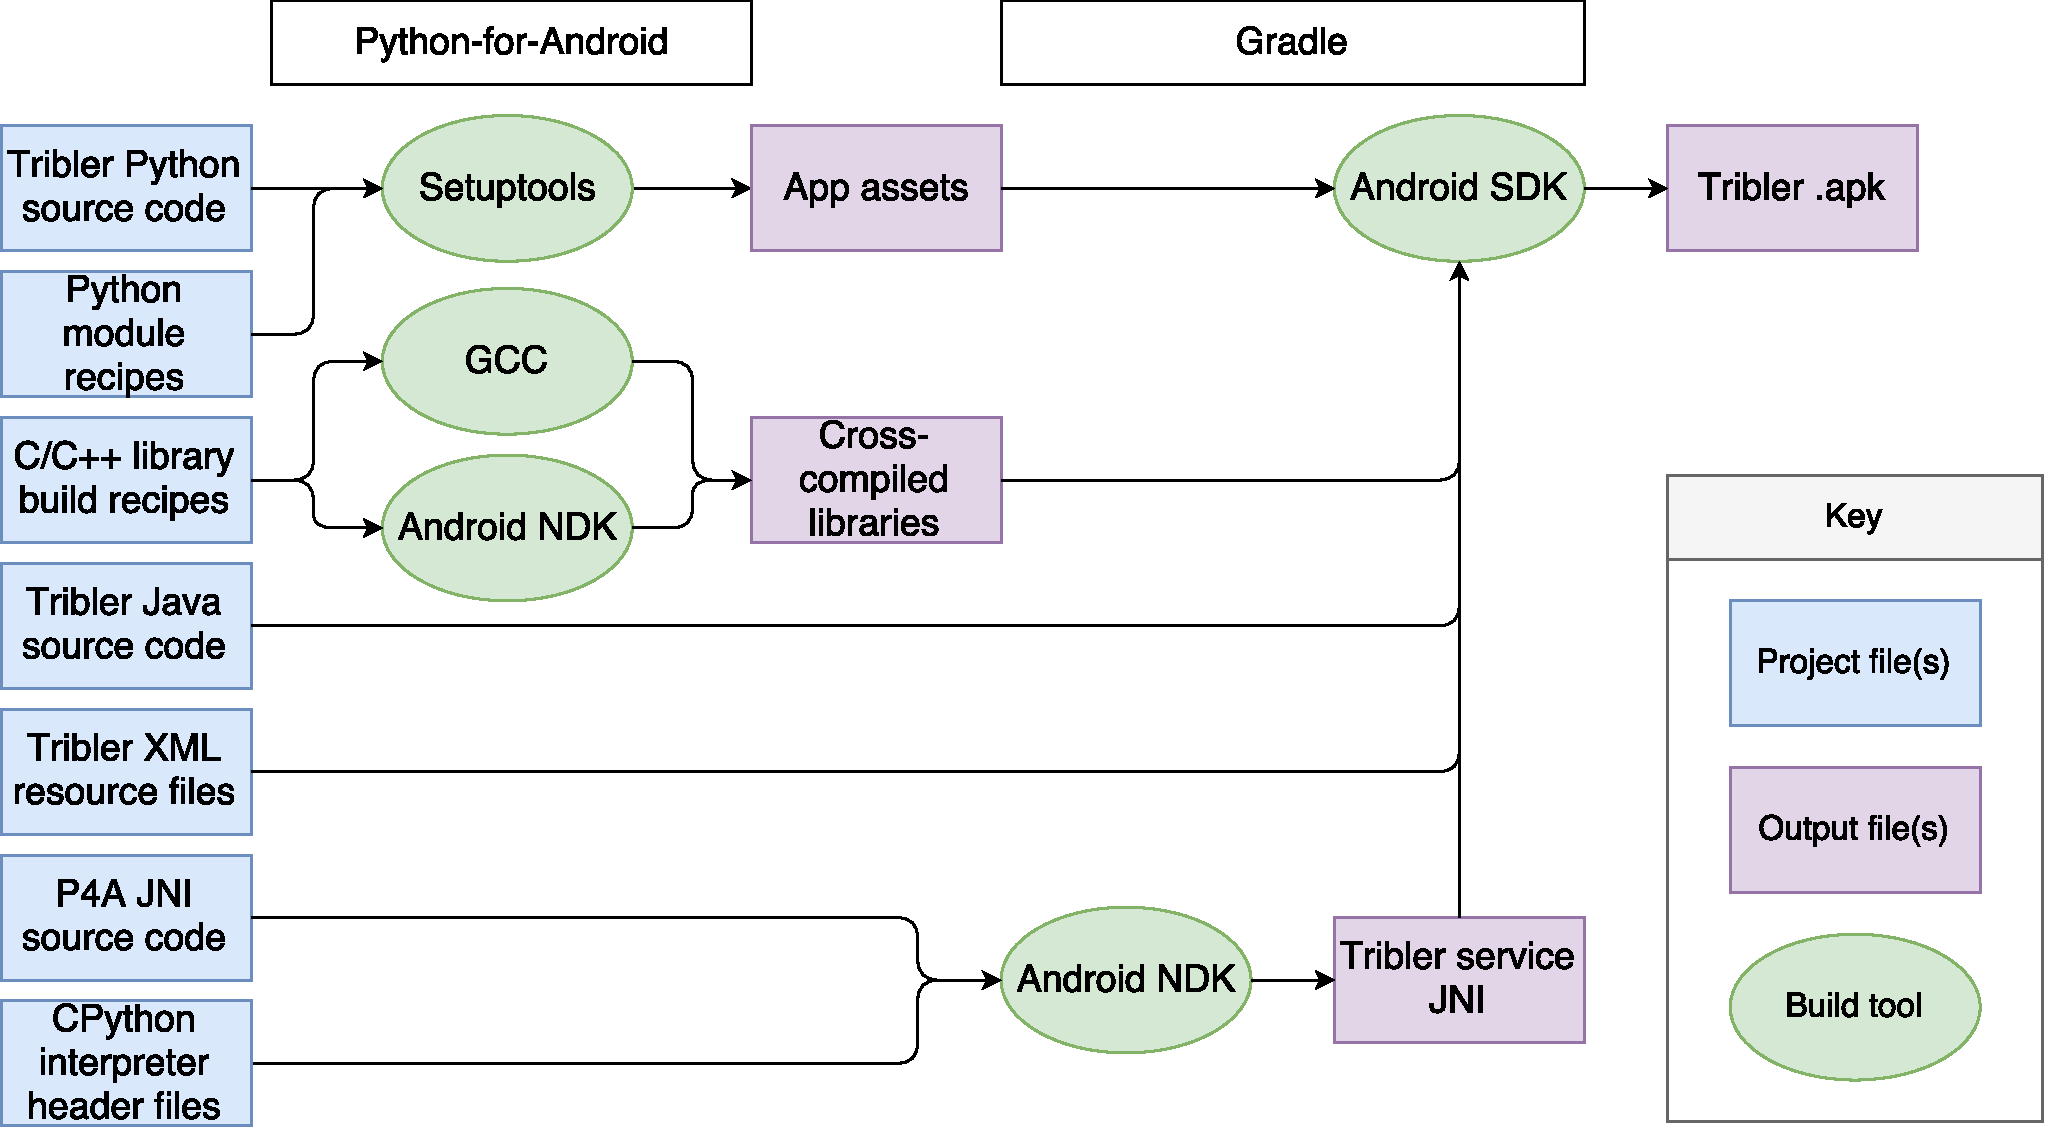
\includegraphics[width=\textwidth]{build_tool_chain}
	\caption{High level overview of the build tool-chain}
	\label{fig:build_tool_chain}
\end{figure}

The libraries are compiled for any ARMv7 compatible platform, and little effort is required to replace Android with another OS in this respect.

%TODO: Link sys arch to build-toolchain


\section{Implementation statistics}\label{sec:impl_stats}
All requirements have been met.
%TODO software stats, delivered, reference github
%lang aan gewerkt
The implementation consists of:
12.806 + X lines of code in the Tribler repository in 35 pull requests and
Y lines of code in the Python-for-Android (P4A) repository in 46 pull requests and
2 lines of code in the M2Crypto repository in 1 pull request.
This excludes the work of reviving the old P4A toolchain.

%TODO: Stats fill-in
Of the X lines (x \%) consists of unit testing code.
Y lines (y \%) is made up of Android specific libraries, and the remainder is..
Table \ref{table:loc}X shows the 25 largest source file contributions for this thesis work. 

\begin{table}
	\begin{tabular}{l | l | l} \hline
		LOC & File & Path \\ \hline \hline
		718 &		MainActivity.java &		.../org/tribler/android/MainActivity.java \\ \hline
		666 &		MyChannelFragment.java &		.../org/tribler/android/MyChannelFragment.java \\ \hline
		482 &		MyUtils.java &		.../org/tribler/android/MyUtils.java \\ \hline
		403 &		DefaultInteractionListFragment.java &		.../org/tribler/android/DefaultInteractionListFragment.java \\ \hline
		318 &		start.c &		android/TriblerApp/app/src/main/jni/src/start.c \\ \hline
		314 &		TriblerViewAdapter.java &		.../org/tribler/android/TriblerViewAdapter.java \\ \hline
		281 &		build.gradle &		android/TriblerApp/app/build.gradle \\ \hline
		256 &		IRestApi.java &		.../org/tribler/android/restapi/IRestApi.java \\ \hline
		234 &		ChannelFragment.java &		.../org/tribler/android/ChannelFragment.java \\ \hline
		186 &		AssetExtract.java &		.../org/kivy/android/AssetExtract.java \\ \hline
		182 & 		BeamActivity.java &		.../org/tribler/android/BeamActivity.java \\ \hline
		175 &		ListFragment.java &		.../org/tribler/android/ListFragment.java \\ \hline
		172 &		CopyFilesActivity.java &		.../org/tribler/android/CopyFilesActivity.java \\ \hline
		166 &		AndroidManifest.xml &		android/TriblerApp/app/src/main/AndroidManifest.xml \\ \hline
		166 &		EventStreamCallback.java &		.../org/tribler/android/restapi/EventStreamCallback.java \\ \hline
		155 &		ChannelActivity.java &		.../org/tribler/android/ChannelActivity.java \\ \hline
		150 &		ViewFragment.java &		.../org/tribler/android/ViewFragment.java \\ \hline
		149 &		PythonService.java & 		.../org/kivy/android/PythonService.java \\ \hline
		149 &		SearchActivity.java &		.../org/tribler/android/SearchActivity.java \\ \hline
		141 &		EditChannelActivity.java &		.../org/tribler/android/EditChannelActivity.java \\ \hline
		131 &		FilterableRecyclerViewAdapter.java &		.../org/tribler/android/FilterableRecyclerViewAdapter.java \\ \hline
		130 & 		BaseActivity.java &		.../org/tribler/android/BaseActivity.java \\ \hline
		114 &		SearchFragment.java &		.../org/tribler/android/SearchFragment.java \\ \hline
		112 & 		TriblerDownload.java &		.../org/tribler/android/restapi/json/TriblerDownload.java \\ \hline
	\end{tabular}
	\caption{Top 25 of largest source file contributions.}
	\label{table:loc}
\end{table}

Code coverage and testing details are further explained in chapter \ref{ch:results}.


